%% LaTeX-Beamer template for KIT design
%% by Erik Burger, Christian Hammer
%% title picture by Klaus Krogmann
%%
%% version 2.1
%%
%% mostly compatible to KIT corporate design v2.0
%% http://intranet.kit.edu/gestaltungsrichtlinien.php
%%
%% Problems, bugs and comments to
%% burger@kit.edu

\documentclass[18pt]{beamer}

%% SLIDE FORMAT

% use 'beamerthemekit' for standard 4:3 ratio
% for widescreen slides (16:9), use 'beamerthemekitwide'

\usepackage{templates/beamerthemekit}
% \usepackage{templates/beamerthemekitwide}
\usepackage{graphicx}
\usepackage{csquotes}
%% TITLE PICTURE

% if a custom picture is to be used on the title page, copy it into the 'logos'
% directory, in the line below, replace 'mypicture' with the 
% filename (without extension) and uncomment the following line
% (picture proportions: 63 : 20 for standard, 169 : 40 for wide
% *.eps format if you use latex+dvips+ps2pdf, 
% *.jpg/*.png/*.pdf if you use pdflatex)

%\titleimage{mypicture}

%% TITLE LOGO

% for a custom logo on the front page, copy your file into the 'logos'
% directory, insert the filename in the line below and uncomment it

%\titlelogo{mylogo}

% (*.eps format if you use latex+dvips+ps2pdf,
% *.jpg/*.png/*.pdf if you use pdflatex)

%% TikZ INTEGRATION

% use these packages for PCM symbols and UML classes
\usepackage{templates/tikzkit}
\usepackage{templates/tikzuml}
\usepackage{amsmath}
\usepackage{MnSymbol}
\usepackage[ruled]{algorithm2e}

% the presentation starts here

\title[Graphen 3]{ICPC}
\subtitle{Graphen 3}
\author{Tobias, Julian, Jakob, Tobias}

\institute{ITI Wagner, IPD Tichy}

% Bibliography

\usepackage[citestyle=authoryear,bibstyle=numeric,hyperref,backend=biber]{biblatex}
\addbibresource{templates/example.bib}
\bibhang1em

\SetKwRepeat{Do}{do}{while}
\SetKwProg{Fn}{Function}{}{}


\begin{document}
	
	% change the following line to "ngerman" for German style date and logos
	\selectlanguage{ngerman}
	
	%title page
	\begin{frame}
	\titlepage
\end{frame}

\section{Einf\"uhrung}

\subsection{Idee: Flussnetzwerk}
\begin{frame}{Idee: Flussnetzwerke}
	\begin{block}{Idee}
		\begin{itemize}
			\visible<1->{\item Transport von Material von einer Quelle zu einer Senke}
			\visible<2->{\item Materialfluss durch Kan\"ale}  
			\visible<3->{\item Mehrere Kan\"ale mit verschiedenen Kapazit\"aten}
			\visible<4->{\item Kanten k\"onnen sich verzweigen und zusammenf\"ugen}
		\end{itemize}
	\end{block}
\end{frame}

\subsection{Einf\"uhrung Flussnetzwerk}
\begin{frame}{Einf\"uhrung Flussnetzwerk}
	\begin{figure}
		\centering
		\begin{tikzpicture}[node distance=2cm, auto, thick]
		
			
			\only<1>{\node[state] (s) {$q_1$}; 
				\node[state, above right = of s] (q0) {$q_0$};
				\node[state, below right = of s] (q1) {$q_3$};
				\node[state, below right = of q0] (t) {$q_2$};}
			
			\visible<2->{\node[state] (s) {$q_0$};
				\node[state, above right = of s, fill=lightgray] (q0) {$s$};
				\node[state, below right = of s, fill=lightgray] (q1) {$t$};
				\node[state, below right = of q0] (t) {$q_1$};}
			
			\path 
				(q0) edge[->,bend left = -20, left] node {30} (s)
				(s) edge[->,bend left = -20, left] node {70} (q1)
				%(q0) edge[->,bend left = 10] node {5} (q1)
				(q0) edge[->,bend right = -20, right] node {60} (t)
				(t) edge[->,bend right = -20, right] node {25} (q1);
			\visible<3-8>{
				\path(q0) edge[->, bend left = 20, red] node {30} (s);}
			\visible<4-8>{
				\path(s) edge[->, bend left = 20, red] node {30} (q1);}
			\visible<5->{
				\path(q0) edge[->, dashed,out=180, in=180, looseness=2, red, left] node {30} (q1);}
			\visible<6-8>{
				\path(q0) edge[->, bend right = 30, red] node {60} (t);}
			\visible<7-8>{
				\path(t) edge[->, bend right = 30, red] node {25} (q1);}
			\visible<8->{
				\path(q0) edge[->, dashed,out = 0, in = 0, looseness = 2, red, right] node {25} (q1);}
			\visible<9->{
				\path (t) edge[->, bend right = 10, black, above left] node {60} (s);}
			\only<10>{
				\path
				(q0) edge[->, bend right = 10,  red, right] node {} (t)
				(t) edge[->, bend left = 10,  red] node {} (s)
				(s) edge[->, bend left = 10, red, right] node {} (q1);}
			\visible<11->{
				\path
				(q0) edge[->, bend right = 10,  red, right] node {35} (t);}
			\visible<12->{
				\path
				(t) edge[->, bend left = 10,  red, below left] node {60} (s)
				(s) edge[->, bend left = 10, red, right] node {40} (q1);}
			\visible<13->{
				\path (q0) edge[->, dashed, red] node {35} (q1);}
			
		\end{tikzpicture}		
	\end{figure}
	
	\centering
	\only<1-2>{
		\begin{block}{\only<1-2>{Gegeben gerichteter Graph}}
				\only<2>{s: source \newline t: sink}
		\end{block} 	
	}
	\only<3-11>{
	\begin{block}{Fluss}
		\only<3>{Kapazit\"atskonfirmit\"at}
		\only<4>{Flusserhaltung}
		\only<5>{Wert eines s-t-Flusses}
		\only<9>{
			Kapazit\"atskonfirmit\"at \newline
			Flusserhaltung\newline 
			Wert eines s-t-Flusses}
		\only<11>{Exzess: Werte entsprechend der Kantenkapazit\"at abz\"uglich bereits vorhandener Fl\"usse}
	\end{block} 
	}
\end{frame}

\section{Max-Flow Algorithmen}
\begin{frame}{Bestimmung des maximalen Flusses}
Idee:
\begin{itemize}
	\item Starte mit dem leeren Fluss
	\item Bestimme erweiternden Pfad (augmenting path) $P$
	\begin{itemize}
		\item[$\Rightarrow$] Ein erweiternder Pfad ist ein einfacher Pfad, der nur Kanten mit positiver Kapazit\"at enth\"alt
	\end{itemize}
	\item Erweitere die L\"osung um $P$
	\item Wiederhole so oft, wie es einen passenden Pfad $P$ gibt 
\end{itemize} 
\vspace{5mm}
\pause 
Frage: Wie kann $P$ gefunden werden?
\end{frame}

\subsection{Ford-Fulkerson}
\begin{frame}{Ford-Fulkerson Algorithmus}
\begin{itemize}
	\item Greedy-Algorithmus, ver\"offentlicht 1956 von L. R. Ford, Jr. und D. R. Fulkerson
	\item Verwendet Tiefensuche, um den erweiternden Pfad $P$ zu bestimmen
\end{itemize}
\end{frame}

\begin{frame}{Ford-Fulkerson Algorithmus}
\begin{itemize}
	\item Die L\"osung wird um $P$ erweitert, indem
	\begin{itemize}
		\pause
		\item die geringste Kapazit\"at $f$ der Kanten in $P$ bestimmt wird
		\pause
		\item die Kapazit\"aten aller Kanten in $P$ um $f$ verringert werden
		\pause
		\item die Kapazit\"aten aller Gegenkanten um $f$ erh\"oht werden
		\pause
		\item der maximale Fluss um $f$ erh\"oht wird
	\end{itemize}  
	\pause
	\item Kapazit\"aten der Gegenkanten werden erh\"oht, um Korrektheit des Algorithmus zu sichern
	\pause
	\begin{itemize}
		\item[$\Rightarrow$] Dies erm\"oglicht, dass diese Gegenkanten in zuk\"unftigen erweiternden Pfaden enthalten sind
		\pause
		\item[$\Rightarrow$] Zuk\"unftige Iterationen k\"onnen den f\"alschlicherweise genutzten Fluss einer Vorw\"artskante wieder (teilweise) umkehren
	\end{itemize}
\end{itemize}
\end{frame}

\begin{frame}{Ford-Fulkerson Algorithmus}
\begin{figure}
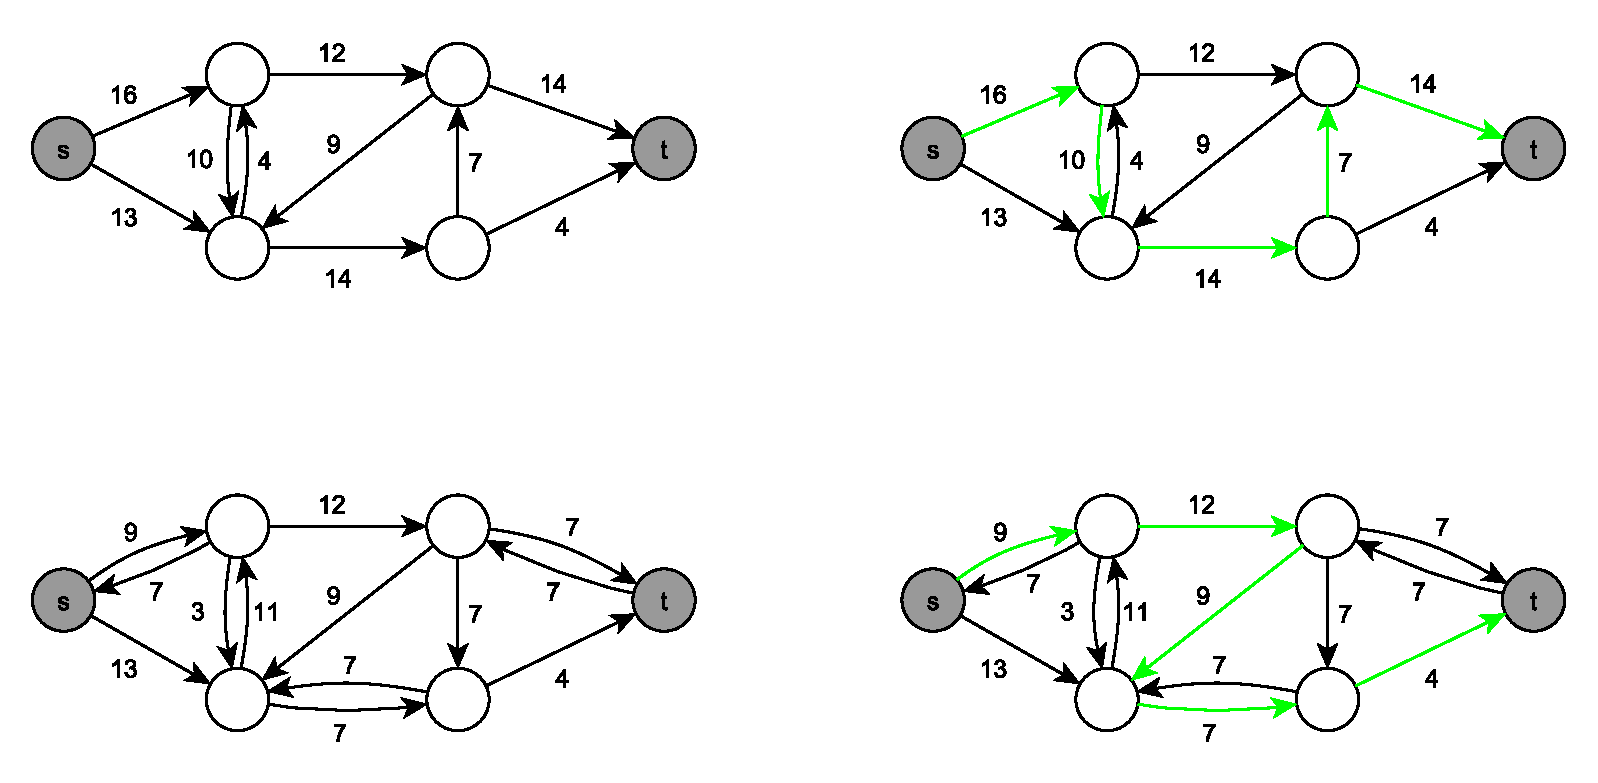
\includegraphics[width = \textwidth]{img/Jakob_Ford.pdf}
\end{figure}
\end{frame}

\begin{frame}{Ford-Fulkerson Algorithmus}
\begin{figure}
	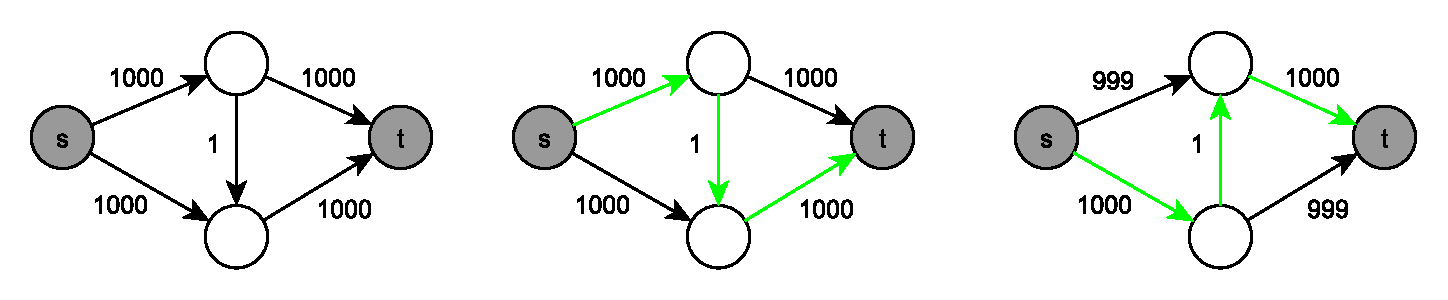
\includegraphics[width = \textwidth]{img/Jakob_Ford2.pdf}
\end{figure}
\end{frame}


\begin{frame}{Ford-Fulkerson Algorithmus}
\begin{figure}
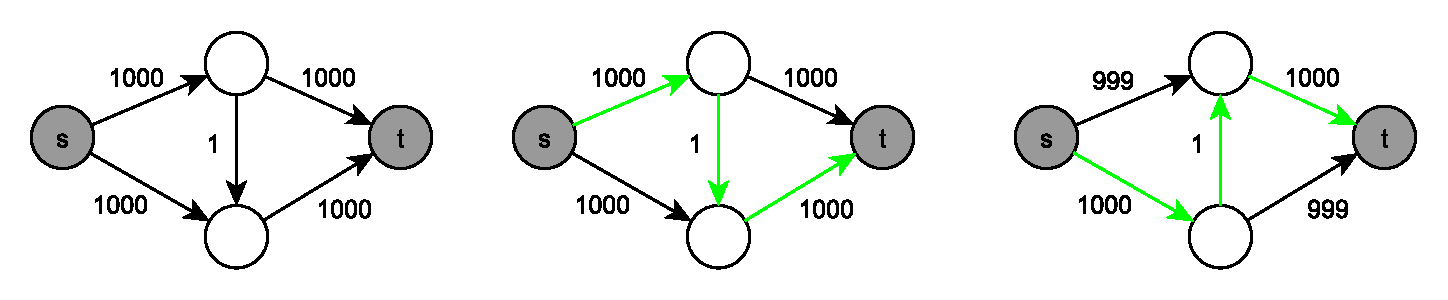
\includegraphics[width = \textwidth]{img/Jakob_Ford3.pdf}
\end{figure}
\begin{itemize}
	\item Im Worst-Case wird der maximale Fluss pro Iteration nur um 1 erh\"oht
	\item[$\Rightarrow$]  Laufzeit in $\mathcal O(|f^*|\cdot |E|)$, wobei $|f^*|$ den Wert des maximalen Flusses beschreibt
	\item Deshalb \textbf{nicht} f\"ur ICPC-Aufgaben geeignet!
\end{itemize}
\end{frame}

\subsection{Edmonds-Karp}
\begin{frame}{Edmonds-Karp Algorithmus}
\begin{itemize}
\item 1972 von J. Edmonds und R. M. Karp ver\"offentlicht
\item Verwendet Breitensuche, um den k\"urzesten erweiternden Pfad $P$ zu bestimmen
\item Erweiterung der L\"osung um $P$ analog zu Ford-Fulkerson
\item Die L\"ange des erweiternden Pfades ist monoton steigend
\item Es sind maximal $|V|\cdot |E|$ Iterationen notwendig
\item[$\Rightarrow$] Laufzeit in $\mathcal O(|V| \cdot |E|^2)$
\end{itemize}
\end{frame}

\begin{frame}{Edmonds-Karp Implementierung}
\SetEndCharOfAlgoLine{}
\begin{algorithm}[H]
	\Fn{Max-Flow (G = (V, E), s, t $\in V$, $c: E \to \mathbb{R}^+$)}{
		$maxFlow = 0 $ \;
		\Do{P exists}{
			find augmenting path P using BFS\;
			$ f = min \{c(u,v) | (u,v) \in P\}$\;
			\ForEach{$(u,v) \in P$}{
				 c(u,v) -= f  \;
				 c(v,u) += f  \;
			}
			maxFlow += f \;
		}
		\textbf{return} maxFlow \;
	}
	\caption{Edmonds-Karp}
\end{algorithm}
\end{frame}

\begin{frame}{Edmonds-Karp Algorithmus}
\begin{figure}
	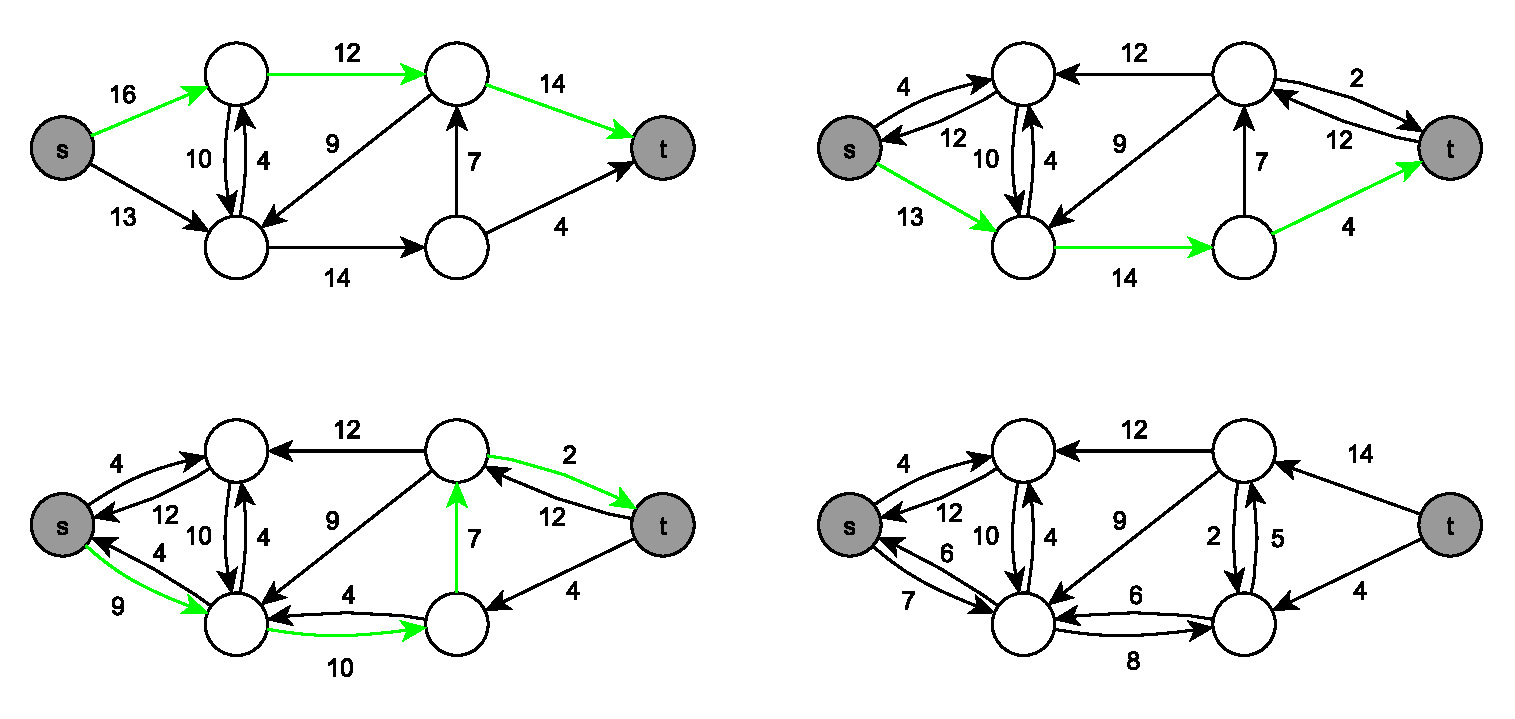
\includegraphics[width = \textwidth]{img/Jakob_Edmond.pdf}
\end{figure}
\end{frame}

\begin{frame}{Edmonds-Karp Implementierungsdetails}
\begin{itemize}
	\item In Adjazenzliste neben Zielknoten auch Kapazit\"at und Verweis auf die R\"uckkante speichern
	\item Nicht vorhandene R\"uckkanten mit 0 initialisieren und dem Graphen hinzuf\"ugen
	\item Bei der Breitensuche nur Kanten mit positiver Kapazit\"at ber\"ucksichtigen
	\item Breitensuche abbrechen, sobald $t$ erreicht wurde
\end{itemize}
\end{frame}


\section{Min-Cut}
\begin{frame}{Min-Cut}
\begin{block}{Min-Cut}

\begin{itemize}
\item Definiere Schnitt \(C = (S, T)\) als Partition von \(V\), wobei \(s \in S\) und \(t \in T\) 
\item $c: E \to \mathbb{R}^+$ eine Kostenfunktion.
\item Weiter sei die Schnittmenge \(cs = \{(u, v) \in E | u \in S \land v \in T\}\)
\item Minimiere nun: 
\begin{equation*}
	\displaystyle \sum_{e\in cs}^{} c(e)
\end{equation*} 
\end{itemize}
\end{block}
\end{frame}

\begin{frame}{Max-Flow-Min-Cut-Theorem}
\begin{block}{Max-Flow-Min-Cut-Theorem}
\begin{itemize}
\item Ein maximaler Fluss hat genau den Wert eines minimalen Schnitts.
\end{itemize}
\end{block}
\end{frame}

\begin{frame}{Max-Flow-Min-Cut}
\begin{itemize}
\item Bsp.:
\end{itemize}
\begin{center}
\begin{tikzpicture}[node distance=2cm, auto, thick]
\node[state, fill=lightgray] (s) {$s$};
\node[state, right=of s] (q0) {$q_0$};
\node[state, below=of s] (q1) {$q_1$};
\node[state, below=of q0, fill=lightgray] (t) {$t$};

\path (s) edge[->,bend left = 10] node {30} (q0)
(s) edge[->,bend left = 10] node {70} (q1)
(q0) edge[->,bend left = 10] node {30} (s)
(q0) edge[->,bend left = 10] node {5} (q1)
(q0) edge[->,bend left = 10] node {70} (t)
(q1) edge[->,bend left = 10] node {70} (s)
(q1) edge[->,bend left = 10] node {5} (q0)
(q1) edge[->,bend left = 10] node {25} (t)
(t) edge[->,bend left = 10] node {70} (q0)
(t) edge[->,bend left = 10] node {25} (q1);
\end{tikzpicture}
\begin{tikzpicture}[node distance=2cm, auto, thick]
\node[state, fill=lightgray] (s) {$s$};
\node[state, right=of s] (q0) {$q_0$};
\node[state, below=of s] (q1) {$q_1$};
\node[state, below=of q0, fill=lightgray] (t) {$t$};

\path (s) edge[->,bend left = 10, dashed, color=blue] node {0} (q0)
(s) edge[->,bend left = 10, dashed] node {40} (q1)
(q0) edge[->,bend left = 10] node {60} (s)
(q0) edge[->,bend left = 10] node {10} (q1)
(q0) edge[->,bend left = 10, dashed] node {35} 	(t)
(q1) edge[->,bend left = 10] node {100} (s)
(q1) edge[->,bend left = 10, dashed, color=blue] node {0} (q0)
(q1) edge[->,bend left = 10, dashed, color=blue] node {0} (t)
(t) edge[->,bend left = 10] node {105} (q0)
(t) edge[->,bend left = 10] node {50} (q1);
\end{tikzpicture}
\end{center}
\begin{itemize}
\item Hier
\begin{itemize}
\item \(C=(\{s,q_1\}, \{t, q_0\})\)
\item \(c=\{(s,q_0), (q_1,q_0), (q_1, t)\}\) 
\end{itemize} 
\end{itemize}
\end{frame}

\section{Sonderf\"alle}
\begin{frame}{Multi-Quelle/Multi-Abfluss}
\begin{itemize}
\item Gegeben sei folgende Situation:
\end{itemize}
\begin{center}
\begin{tikzpicture}[auto, thick]
\node[state, fill=lightgray] (s1) {$s$};
\node[state, below=of s, fill=lightgray] (s2) {$s$};
\node[state] (q1) at (2,-1) {};
\node[state, fill=lightgray] (t1) at (4,0) {$t$};
\node[state, below=of t1, fill=lightgray] (t2) {$t$};

\path (s1) edge[->] node {} (q1)
(s2) edge[->] node {} (q1)
(q1) edge[->] node {} (t1)
(q1) edge[->] node {} (t2);
\end{tikzpicture}
\end{center}
\begin{itemize}
\item Problem: Max-Flow Algorithmus kann nur mit einer Quelle und einer Senke arbeiten.
\item L\"osung: Ertelle Super-Quelle und Super-Senke und verbinde alle Quellen und Senken mit Kantengewicht $\infty$
\end{itemize}
\end{frame}

\begin{frame}{Multi-Quelle/Multi-Abfluss L\"osung}
\begin{center}
\begin{tikzpicture}[auto, thick]
\node[state, fill=lightgray] (ss) at (-2,-1) {$ss$};
\node[state] (s1) {$s$};
\node[state, below=of s] (s2) {$s$};
\node[state] (q1) at (2,-1) {};
\node[state] (t1) at (4,0) {$t$};
\node[state, below=of t1] (t2) {$t$};
\node[state, fill=lightgray] (st) at (6, -1) {$st$};

\path (s1) edge[->] node {} (q1)
(s2) edge[->] node {} (q1)
(q1) edge[->] node {} (t1)
(q1) edge[->] node {} (t2)
(ss) edge[->] node {$\infty$} (s1)
(ss) edge[->] node {$\infty$} (s2)
(t1) edge[->] node {$\infty$} (st)
(t2) edge[->] node {$\infty$} (st);
\end{tikzpicture}
\end{center}
\end{frame}

\begin{frame}{Knotenkapazit\"at}
\begin{itemize}
\item Gegeben sind Knoten mit Kapazit\"at.
\item Bsp.:
\end{itemize}
\begin{center}
\begin{tikzpicture}[auto, thick]
\node[state] (V) {$V|7$};

\path (V) edge[->] node {5} (1.5,0)
(-1, 1) edge[->] node {10} (V)
(-1, -1) edge[->] node {4} (V);
\end{tikzpicture}
\end{center}
\end{frame}

\begin{frame}{Knotenkapazit\"at}
\begin{itemize}
\item Gegeben sind Knoten mit Kapazit\"at.
\item Bsp.:
\end{itemize}
\begin{center}
\begin{tikzpicture}[auto, thick]
\node[state] (V1) {$V_{in}$};
\node[state, right=of V1] (V2) {$V_{out}$};

\path (V1) edge[->] node {7} (V2)
(-1, 1) edge[->] node {10} (V1)
(-1, -1) edge[->] node {4} (V1)
(V2) edge[->] node {5} (3.5, 0);
\end{tikzpicture}
\end{center}
\end{frame}

\section{Max-Flow Modellierung}
\begin{frame}{Modellierung}
\begin{itemize}
\item Erkennen eines Netzwerkfluss-Problems nicht immer einfach
\pause
\item Was hilft?
\begin{itemize}
\pause
\item \"Ubung
\item \"Ubung
\item ...
\end{itemize}
\end{itemize}
\end{frame}

\begin{frame}{Modellierung - Beispiel}
\begin{itemize}
\item Situation: Die Titanic ist gesunken. Es soll ermittelt werden, wie viele Menschen gerettet werden k\"onnen.
\item Eingabe: $X$, $Y$, $P$ mit $X$,$Y$ Dimension der Fl\"ache (\(1 \leq X,Y \leq 30\)) und $P$ (\(P \leq 10\)) die Anzahl von Personen, welche gleichzeitig auf ein Holzbrett k\"onnen.
\end{itemize}
\begin{center}
\begin{tabular}{c|l}
Symbol & Bedeutung \\
\hline
* & Menschen auf Treibeis \\
\(\sim\) & Eiskaltes Wasser \\
. & Treibeis \\
@ & Gro\ss er Eisberg \\
\# & Gro\ss es Holzbrett \\
\end{tabular}
\end{center}
\end{frame}

\begin{frame}{Modellierung - Beispiel}
\begin{itemize}
\item Gegeben sei nun folgende Eingabe:
\end{itemize}
\begin{center}
\begin{tabular}{cccc}
* & \(\sim\) & \(\sim\) & \# \\
. & . & . & @ \\
. & \(\sim\) & . & * \\
\end{tabular}
\end{center}
\begin{itemize}
\pause\item Wandle in Graphen um...
\end{itemize}
\end{frame}

\begin{frame}{Modellierung - Beispiel}
\begin{center}
\begin{tikzpicture}[auto, thick]
\node[state] (1) {$*$};
\node[state, right=of 1] (2) {\(\sim\)};
\node[state, right=of 2] (3) {\(\sim\)};
\node[state, right=of 3] (4) {\#};
\node[state, below=of 1] (5) {$.$};
\node[state, right=of 5] (6) {$.$};
\node[state, right=of 6] (7) {$.$};
\node[state, right=of 7] (8) {@};
\node[state, below=of 5] (9) {$.$};
\node[state, right=of 9] (10) {\(\sim\)};
\node[state, right=of 10] (11) {$.$};
\node[state, right=of 11] (12) {$*$};
\end{tikzpicture}
\end{center}
\begin{itemize}
\pause
\item Verbinde alle Knoten, \"uber die ein Weg m\"oglich ist...
\end{itemize}
\end{frame}

\begin{frame}{Modellierung - Beispiel}
\begin{center}
\begin{tikzpicture}[auto, thick]
\node[state] (1) {$*$};
\node[state, right=of 1] (2) {\(\sim\)};
\node[state, right=of 2] (3) {\(\sim\)};
\node[state, right=of 3] (4) {\#};
\node[state, below=of 1] (5) {$.$};
\node[state, right=of 5] (6) {$.$};
\node[state, right=of 6] (7) {$.$};
\node[state, right=of 7] (8) {@};
\node[state, below=of 5] (9) {$.$};
\node[state, right=of 9] (10) {\(\sim\)};
\node[state, right=of 10] (11) {$.$};
\node[state, right=of 11] (12) {$*$};

\path (1) edge[-] node {} (5)
(5) edge[-] node {} (6)
(5) edge[-] node {} (9)
(6) edge[-] node {} (7)
(7) edge[-] node {} (8)
(7) edge[-] node {} (11)
(8) edge[-] node {} (4)
(8) edge[-] node {} (12);
\end{tikzpicture}
\end{center}
\begin{itemize}
\pause
\item F\"uge Knotengewichte hinzu...
\end{itemize}
\end{frame}

\begin{frame}{Modellierung - Beispiel}
\begin{center}
\begin{tikzpicture}[auto, thick]
\node[state] (1) {$*|1$};
\node[state, right=of 1] (2) {\(\sim\)};
\node[state, right=of 2] (3) {\(\sim\)};
\node[state, right=of 3] (4) {\# $|1000$};
\node[state, below=of 1] (5) {$.|1$};
\node[state, right=of 5] (6) {$.|1$};
\node[state, right=of 6] (7) {$.|1$};
\node[state, right=of 7] (8) {@$|1000$};
\node[state, below=of 5] (9) {$.|1$};
\node[state, right=of 9] (10) {\(\sim\)};
\node[state, right=of 10] (11) {$.|1$};
\node[state, right=of 11] (12) {$*|1$};

\path (1) edge[-] node {} (5)
(5) edge[-] node {} (6)
(5) edge[-] node {} (9)
(6) edge[-] node {} (7)
(7) edge[-] node {} (8)
(7) edge[-] node {} (11)
(8) edge[-] node {} (4)
(8) edge[-] node {} (12);
\end{tikzpicture}
\end{center}
\begin{itemize}
\pause
\item Verbinde alle Menschen mit s und alle Holzbretter mit t...
\end{itemize}
\end{frame}

\begin{frame}{Modellierung - Beispiel}
\begin{center}
\begin{tikzpicture}[auto, thick]
\node[state] (1) {$*|1$};
\node[state, right=of 1] (2) {\(\sim\)};
\node[state, right=of 2] (3) {\(\sim\)};
\node[state, right=of 3] (4) {\# $|1000$};
\node[state, below=of 1] (5) {$.|1$};
\node[state, right=of 5] (6) {$.|1$};
\node[state, right=of 6] (7) {$.|1$};
\node[state, right=of 7] (8) {@$|1000$};
\node[state, below=of 5] (9) {$.|1$};
\node[state, right=of 9] (10) {\(\sim\)};
\node[state, right=of 10] (11) {$.|1$};
\node[state, right=of 11] (12) {$*|1$};

\path (1) edge[-] node {} (5)
(5) edge[-] node {} (6)
(5) edge[-] node {} (9)
(6) edge[-] node {} (7)
(7) edge[-] node {} (8)
(7) edge[-] node {} (11)
(8) edge[-] node {} (4)
(8) edge[-] node {} (12);

\node[state, left=of 5] (s) {$s$};
\node[state, right=of 8] (t) {$t$};

\path (s) edge[->] node {1} (1)
(s) edge[->] node {1} (12)
(4) edge[->] node {P} (t);
\end{tikzpicture}
\end{center}
\begin{itemize}
\item Bem.: Knotengewichte m\"ussen noch aufgel\"ost werden
\end{itemize}
\end{frame}

\section{Bipartite Matching}
\begin{frame}{Bipartiter Graph}
\begin{block}{Bipartiter Graph}
\begin{itemize}
\item Ein Graph G = (V, E) hei{\ss}t \textbf{bipartit}, wenn sich $V = A \cupdot B$ in 2 disjunkte Knotenmengen A und B aufteilen l\"asst,
sodass zwischen den Knoten innerhalb der Teilmengen keine Kanten existieren.
\end{itemize}
\end{block}
\end{frame}

\begin{frame}{Bipartiter Graph}
\begin{center}
\begin{tikzpicture}[auto, thick]
\node[state] (1) at (1, 1) {$a_{1}$};
\node[state] (2) at (3, 1) {$a_{2}$};
\node[state] (3) at (5, 1) {$a_{3}$};
\node[state] (4) at (7, 1) {$a_{4}$};
\node[state] (5) at (2, 4) {$b_{1}$};
\node[state] (6) at (4, 4) {$b_{2}$};
\node[state] (7) at (6, 4) {$b_{3}$};

\path
(1) edge[-] node {} (5)
(2) edge[-] node {} (5)
(2) edge[-] node {} (6)
(3) edge[-] node {} (6)
(3) edge[-] node {} (7)
(4) edge[-] node {} (6)
(4) edge[-] node {} (7);

\draw[thick, dashed, color=red] (0,0) rectangle (8,2);
\draw[thick, dashed, color=green] (1,3) rectangle (7,5);

\end{tikzpicture}
\end{center}
\end{frame}

\begin{frame}{Matching}
\begin{block}{Matching}
\begin{itemize}
\item Sei $G = (V, E)$ ein Graph. Ein \textbf{Matching} $M \subseteq E$ ist eine Menge paarweise knotendisjunkter Kanten,
d.h. $\forall e_{1} = \{u_{1}, v_{1}\}, e_{2} = \{u_{2}, v_{2}\} \in M, e_{1} \neq e_{2}: e_{1} \cap e_{2} = \emptyset$
\item Analog f\"ur gerichtete Graphen
\end{itemize}
\end{block}

\pause

\begin{block}{Maximales Matching}
\begin{itemize}
\item Ein Matching hei{\ss}t \textbf{maximales Matching}, wenn nicht durch Hinzuf\"ugen einer Kante ein gr\"o{\ss}eres Matching erstellt werden kann.
(D.h. es gibt keine Kante $e = \{u, v\}$, wobei $u$ und $v$ nicht Teil des Matchings sind.)
\end{itemize}
\end{block}
\end{frame}

\begin{frame}{Mehr Matchings}
\begin{block}{Kardinalit\"atsmaximales Matching}
\begin{itemize}
\item Ein Matching $M \subseteq E$ hei{\ss }t \textbf{kardinalit\"atsmaximales Matching}, wenn es kein gr\"o{\ss}eres Matching gibt.
(D.h. $\forall$ Matchings $M': |M| \geq |M'|$).
\end{itemize}
\end{block}

\pause

\begin{block}{Perfektes Matching}
\begin{itemize}
\item Ein Matching $M$ hei{\ss}t \textbf{perfekt}, falls $2 \cdot |M| = |V|$, d.h. jeder Knoten $v \in V$ kommt in $M$ vor.
\end{itemize}
\end{block}
\end{frame}

\begin{frame}{Beispiel: Matching (\textit{nicht bipartit})}
\begin{center}
\begin{tikzpicture}[auto, thick]

\visible<1-2>{
\node[state] (1) at (3, 7) {};
}
\node[state] (2) at (1, 5) {};
\node[state] (3) at (3, 5) {};
\node[state] (4) at (5, 5) {};
\node[state] (5) at (1, 3) {};
\node[state] (6) at (3, 3) {};
\node[state] (7) at (5, 3) {};

\path
(2) edge[-] node {} (5)
(2) edge[-] node {} (6)
(3) edge[-] node {} (5)
(3) edge[-] node {} (6)
(4) edge[-] node {} (7)
(5) edge[-] node {} (6)
(6) edge[-] node {} (7);

\visible<1-2>{ \path
(1) edge[-] node {} (7);
}

\only<1>{ \path
(5) edge[-, line width=1.5pt, color=red] node {} (6)
(1) edge[-, line width=1.5pt, color=red] node {} (7);
}
\visible<2-4>{ \path
(4) edge[-, line width=1.5pt, color=red] node {} (7);
}
\visible<2-3>{ \path
(2) edge[-, line width=1.5pt, color=red] node {} (5)
(3) edge[-, line width=1.5pt, color=red] node {} (6);
}
\only<4>{ \path
(2) edge[-, line width=1.5pt, color=red] node {} (6)
(3) edge[-, line width=1.5pt, color=red] node {} (5);
}
\visible<1-2>{ \path
(1) edge[-] node {} (2)
(1) edge[-] node {} (3)
(1) edge[-] node {} (4);
}

\end{tikzpicture}
\end{center}

\centering
\only<1>{Maximales Matching}
\only<2>{Kardinalit\"atsmaximales Matching}
\only<3>{Perfektes Matching}
\only<4>{anderes perfektes Matching}
\end{frame}

\begin{frame}{Beispiel}
\begin{itemize}
\item Gegeben: Menge von Aufgaben $A$, Personen $B$
\item F\"ur jede Person eine Liste von Aufgaben, die diese Person erledigen kann
\item Gesucht: Zuteilung von Aufgaben an Personen, sodass m\"oglichst viele Aufgaben erledigt werden
\item Jede Aufgabe kann von maximal einer Person zugeteilt werden, jeder Person kann maximal eine Aufgabe zugeteilt werden
\pause
\item L\"osung: Modellierung als \textit{bipartiter Graph} mit Knotenmengen $A$ und $B$
\item Kante zwischen Aufgabe $a$ und Person $b$, wenn $b$ Aufgabe $a$ l\"osen kann
\pause
\item L\"osung entspricht \textit{kardinalit\"atsmaximalem Matching}
\end{itemize}
\end{frame}

\begin{frame}{Modellierung}
\begin{center}
\begin{tikzpicture}[auto, thick]
\node[state] (2) at (3, 1) {$a_{4}$};
\node[state] (3) at (3, 3) {$a_{3}$};
\node[state] (4) at (3, 5) {$a_{2}$};
\node[state] (5) at (3, 7) {$a_{1}$};
\node[state] (6) at (6, 2) {$b_{3}$};
\node[state] (7) at (6, 4) {$b_{2}$};
\node[state] (8) at (6, 6) {$b_{1}$};

\visible<2->{
\node[state, fill=lightgray] (1) at (1, 4) {s};
\node[state, fill=lightgray] (9) at (8, 4) {t};
}

\path
(2) edge[->] node {} (6)
(3) edge[->] node {} (6)
(3) edge[->] node {} (8)
(4) edge[->] node {} (6)
(4) edge[->] node {} (7)
(4) edge[->] node {} (8)
(5) edge[->] node {} (6)
(5) edge[->] node {} (7)
(5) edge[->] node {} (8);

\only<2>{ \path
(1) edge[->] node {} (2)
(1) edge[->] node {} (3)
(1) edge[->] node {} (4)
(1) edge[->] node {} (5)
(6) edge[->] node {} (9)
(7) edge[->] node {} (9)
(8) edge[->] node {} (9);
}

\only<3>{ \path
(1) edge[->] node {} (2)
(1) edge[->, color=red] node {} (3)
(1) edge[->, color=red] node {} (4)
(1) edge[->, color=red] node {} (5)
(3) edge[->, line width=1.5pt, color=red] node {} (6)
(4) edge[->, line width=1.5pt, color=red] node {} (7)
(5) edge[->, line width=1.5pt, color=red] node {} (8)
(6) edge[->, color=red] node {} (9)
(7) edge[->, color=red] node {} (9)
(8) edge[->, color=red] node {} (9);
}
\end{tikzpicture}
\end{center}
\end{frame}

\begin{frame}{Modellierung}
\begin{itemize}
\item Finden von kardinalit\"atsmaximalen Matchings in bipartiten Graphen $G = (V, E = A \cupdot B)$:
\begin{itemize}
	\item Einf\"ugen von neuen Knoten $s$ und $t$
	\item Einf\"ugen von Kanten zwischen $s$ und allen Knoten $v_{A} \in A$, und zwischen allen Knoten $v_{B} \in B$ und $t$.
	\item Jede Kante im Graph (alte und neu eingef\"ugte) hat Kapazit\"at 1.
	\item Berechnen des maximalen Flusses von $s$ nach $t$.
\end{itemize}
\item Kanten des \textit{maximalen Flusses} zwischen $A$ und $B$ entsprechen \textit{kardinalit\"atsmaximalen Matching}.
\item Laufzeit Edmonds-Karp (in diesem Fall): $\mathcal{O}(|E| \cdot |V|)$
\end{itemize}
\end{frame}

\begin{frame}{Mehr Graphentheorie}
\begin{block}{Max Independent Set}
\begin{itemize}
\item Ein \textbf{independent set} $S \subseteq V$ ist eine Menge von Knoten, die paarweise nicht \textit{adjazent} sind,
d.h. $\forall u, v \in S: \{u, v\} \notin E$ (zwischen keinen zwei Knoten existiert eine Kante).
\item Ein \textbf{maximal independent set} ist ein maximal gro{\ss}es \textit{independent set}.
\item Das bedeutet: Jeder Knoten ist entweder selbst in $S$, oder einer seiner Nachbarn ist in $S$.
\end{itemize}
\end{block}

\pause

\begin{block}{Min Vertex Cover}
\begin{itemize}
\item Ein \textbf{vertex cover} $U \subseteq V$ ist eine Menge von Knoten, sodass jede Kante von G zu einem Knoten aus U \textit{inzident} ist,
d.h. $\forall \{v, w\} = e \in E: \exists u \in U: u \in e$.
\item Ein \textbf{minimum vertex cover} ist ein minimal gro{\ss}es \textit{vertex cover}.
\end{itemize}
\end{block}
\end{frame}

\begin{frame}{Noch mehr Graphentheorie}
\begin{block}{Kőnigs Theorem }
\begin{itemize}
\item Sei $G$ ein \textit{bipartiter} Graph, $M$ ein \textit{kadinalit\"atsmaximales Matching}, $U$ ein \textit{minimum vertex cover}.
\item Dann gilt $|M| = |U|$.
\item In Worten: Die Anzahl an Kanten eines kardinalit\"atsmaximalen Matchings entspricht der Anzahl an Knoten in einem minimum vertex cover
\textit{in einem bipartiten Graph}.
\end{itemize}
\end{block}

\pause

\begin{block}{Andere Erkenntnis}
\begin{itemize}
\item In einem bipartiten Graph mit \textit{minimum vertex cover} $U$ und \textit{maximalen independent set} $S$ gilt:
\item $|U| + |S| = |V|$.
\end{itemize}
\end{block}
\end{frame}

\begin{frame}{Veranschaulichung}
\begin{center}
\begin{tikzpicture}[auto, thick]

\draw[thick, fill=lightgray] (0,2) rectangle (2,6);
\draw[thick, fill=gray] (4,0) rectangle (6,6);

\node[state, fill=white] (1) at (1, 3) {$v_{2}$};
\node[state, fill=white] (2) at (1, 5) {$v_{1}$};
\node[state, fill=white] (3) at (5, 1) {$s_{3}$};
\node[state, fill=white] (4) at (5, 3) {$s_{2}$};
\node[state, fill=white] (5) at (5, 5) {$s_{1}$};

\path
(1) edge[-] node {} (3)
(1) edge[-, line width=1.5pt, color=red] node {$m_{1}$} (4)
(2) edge[-, line width=1.5pt, color=red] node {$m_{2}$} (5)
(2) edge[-] node {} (4)
(1) edge[-] node {} (5);

\end{tikzpicture}
\end{center}
\end{frame}

\begin{frame}{Beispiel: Guardian of Decency}
\begin{itemize}
\item Gegeben: N Sch\"uler (mit Gr\"o{\ss}e, Geschlecht, Musikgeschmack, Lieblingssport).
\item Gesucht: Wie viele k\"onnen maximal auf Exkursion gehen, sodass je zwei Sch\"uler kein P\"archen werden k\"onnen, da...
\begin{itemize}
	\item ...sich ihre Gr\"o{\ss}e um mehr als 40 cm unterscheidet,
	\item ...sie das selbe Geschlecht haben,
	\item ...ihr Musikgeschmack unterschiedlich ist,
	\item ...oder sie den selben Lieblingssport haben.
\end{itemize}

\pause

\item Kante zwischen Personen, wenn sie ein P\"archen werden k\"onnten
\item Graph ist bipartit: M\"annliche und weibliche Sch\"uler
\pause
\item Aufgabenstellung: Maximum independent set
\item L\"osung: $|$maximum independent set$| = N - |$kardinalit\"atsmaximales Matching$|$
\end{itemize}
\end{frame}

\begin{frame}{Bonusfolie}
\begin{itemize}
\item Es gilt: $G$ \textit{bipartit} $\Leftrightarrow$ $G$ enth\"alt keine ungeraden Kreise
\begin{itemize}
	\item Damit zum Beispiel bipartit: Jeder Baum
\end{itemize}
\item Sei $G$ \textit{bipartit} mit $V = A \cupdot B$. Dann: $G$ hat \textit{perfektes Matching} $\Leftrightarrow \forall S \subset A: |N(S)| \geq |S|$
(Wobei die Nachbarn $N(S)$ alle zu einem Knoten $s \in S$ adjazenten Knoten sind).
\item Es gibt asymptotisch bessere Algorithmen zum Finden maximaler Fl\"usse, zum Beispiel \textit{Dinitz} ($\mathcal{O}(|V|^{2} \cdot |E|)$) oder Push-Relabel-Algorithmen
\end{itemize}
\end{frame}

\begin{frame}{Bonusbeispiel}
\begin{itemize}
\item Definition: \textit{Complete prime pairing}: Teile Liste $M$ von nat\"urlichen Zahlen so vollst\"andig in Paare auf,
dass die Summe beider Elemente eines Paares immer eine Primzahl ist.
\item Gegeben: Liste $N$ von paarweise unterschiedlichen Zahlen $n_{i} \in \mathbb{N}$.
\item Gesucht: Liste $M \subseteq N$, sodass: $\forall m \in M$:
\begin{itemize}
	\item  $\{m, n_{0}\}$ ist ein prime pair, d.h. $m + n_{0}$ ist prim
	\item $N \setminus \{n_{0}, m\}$ besitzt ein \textit{complete prime pairing}.
\end{itemize}
\pause
\item Erkenntnis: Alle Primzahlen m\"ussen als Summe einer geraden und einer ungeraden Zahl zustande kommen.
\item Damit: Bipartiter Graph, Kante zwischen $a$ und $b$, falls $a + b$ eine Primzahl ist.
\item Falls beide Mengen unterschiedlich gro{\ss} sind, gibt es keine L\"osung
\item Ansonsten: Gehe alle Nachbarn $n'$ von $n_{0}$ durch und \"uberpr\"ufe, ob $G - \{n_{0}, n'\}$ ein \textit{perfektes Matching} hat.
\end{itemize}
\end{frame}

\end{document}
